\documentclass[12pt,letterpaper]{article}
\usepackage[T1]{fontenc}
\usepackage{lmodern,amsmath,amssymb,booktabs,array}
\usepackage[margin=0.87in,top=0.83in,bottom=0.82in,footskip=0.39in]{geometry}
\usepackage{microtype,xcolor,tikz,fancyhdr,hyperref}
\definecolor{ink}{HTML}{182B35}
\definecolor{accent}{HTML}{14675E}
\definecolor{soft}{HTML}{EEF5F2}
\definecolor{muted}{HTML}{526671}
\hypersetup{colorlinks=true,urlcolor=accent,linkcolor=accent,pdftitle={Quadratic reciprocity in intuitionistic primitive recursive arithmetic},pdfauthor={Research note for Vladimir Reshetnikov},pdfsubject={A finite proof and Lean formalization guide}}
\pagestyle{fancy}\fancyhf{}\setlength{\headheight}{15pt}
\fancyhead[L]{\small\sffamily\color{muted}Quadratic reciprocity in iPRA}
\fancyhead[R]{\small\sffamily\color{muted}Number theory}
\fancyfoot[C]{\small\sffamily\color{muted}\thepage}
\renewcommand{\headrulewidth}{0.3pt}
\setlength{\parindent}{0pt}\setlength{\parskip}{5.5pt plus 1pt minus 1pt}
\setlength{\abovedisplayskip}{6pt plus 2pt minus 1pt}\setlength{\belowdisplayskip}{6pt plus 2pt minus 1pt}
\raggedbottom\color{ink}
\newcommand{\sect}[1]{\section{\texorpdfstring{\color{accent}#1}{#1}}}
\newcommand{\lab}[1]{\textbf{#1.}\enspace}
\newcommand{\leg}[2]{\left(\frac{#1}{#2}\right)}
\newcommand{\floor}[1]{\left\lfloor#1\right\rfloor}
\newcommand{\remn}{\operatorname{rem}}
\newcommand{\rootf}{\operatorname{root}}
\newcommand{\sgnbit}{\varepsilon}
\newcommand{\half}{\operatorname{half}}
\newcommand{\iv}[1]{[1,#1]}
\newcommand{\QR}{\mathrm{QR}}
\newcommand{\ipra}{\mathsf{iPRA}}
\newcommand{\code}[1]{\texttt{#1}}
\newcommand{\repo}{https://github.com/VladimirReshetnikov/ProveIt/}
\begin{document}
\thispagestyle{plain}
{\Huge\bfseries\sffamily\color{accent}Quadratic reciprocity}\par
{\LARGE\bfseries in intuitionistic primitive recursive arithmetic}\par
\vspace{3pt}
\textit{A finite proof, its witness functions, and a Lean formalization guide}
\par\vspace{3pt}\hrule\vspace{4pt}
\sect{The theorem as a numerical identity}\label{sec:statement}
Let $p,q$ be distinct odd primes, and put $h=(p-1)/2$, $k=(q-1)/2$. The Legendre symbol $\leg{a}{p}$ is $0$ if $p\mid a$, $+1$ if $a$ is a nonzero square modulo $p$, and $-1$ otherwise. We prove
\begin{equation}\label{eq:qr}
  \boxed{\displaystyle \leg{q}{p}\leg{p}{q}=(-1)^{hk}.}
\end{equation}
Thus $q$ is a square modulo $p$ exactly when $p$ is a square modulo $q$ if at least one prime is $1\bmod 4$. If both are $3\bmod4$, exactly one of these square tests succeeds. We also prove the supplementary laws for $-1$ and $2$.

Here $\ipra$ means intuitionistic first-order arithmetic with defining equations for all primitive recursive (PR) functions, the successor axioms, and quantifier-free induction with parameters. Write $\remn_p(a)$ for the least nonnegative remainder. Roots of an integer numerator are tested on its remainder. For $p>0$, define
\[
 \rootf(p,a)=\text{the least }x<p\text{ with }\remn_p(x^2)=\remn_p(a),
\]
with default $p$ when the scan has no match. Put $\sgnbit_p(a)=[\rootf(p,a)=p]$, where $[P]$ is $1$ if the decidable test $P$ succeeds and $0$ otherwise. Thus $\sgnbit_p(a)=0$ exactly when the scan finds a root, including for a zero numerator. In the unit case $\leg{a}{p}=(-1)^{\sgnbit_p(a)}$.

Let $O(p)$ test $p\ge3$, oddness, and $\remn_d(p)\ne0$ for every $2\le d<p$. Put $H(p)=\floor{(p\mathbin{\dot-}1)/2}$ with truncated subtraction. The actual first-order theorem is the universal closure of
\begin{equation}\label{eq:target}
 O(p)\land O(q)\land p\ne q\ \longrightarrow\ 
 (\sgnbit_p(q)+\sgnbit_q(p))\bmod 2=H(p)H(q)\bmod 2.
\end{equation}
Its matrix is quantifier-free after the displayed computations are named. Distinct primes are units modulo each other. The smaller cannot divide the larger by primality, and the larger cannot divide the positive smaller number. Hence \eqref{eq:target} gives exactly \eqref{eq:qr}.

The proof follows one count through three descriptions. Square roots are fixed points of $x\mapsto a/x$, a sign is the parity of a count of large remainders, and that parity counts one side of a finite rectangle.
\clearpage
\sect{Bounded reasoning and finite rearrangements}\label{sec:bounded}
All computations take natural-number inputs. A remainder at divisor zero may be set to the dividend, and a quotient at divisor zero to zero. The proof uses positive divisors. For $d>0$ one can find the quotient by scanning $0\le t\le n$ for the largest $t$ with $dt\le n$. Then $n=dt+r$, $0\le r<d$. Comparing two such decompositions gives uniqueness. Addition, multiplication, truncated subtraction, comparisons, powers, bounded sums and bounded products all have primitive recursive defining equations. We use ordinary congruence notation for equality of remainders. Modular negation can be computed as $\remn_p(p\mathbin{\dot-}\remn_p(x))$.

\lab{What justifies search} For a fixed PR Boolean test $B(i)$ let $w(t)$ be its first match among $i<t$, with sentinel $t$. Start at $w(0)=0$. On extending to $t+1$, retain $w(t)$ if $w(t)<t$. Otherwise return $t$ if $B(t)$ and $t+1$ if it fails. Quantifier-free induction proves $w(t)\le t$ and $w(t)<t\Rightarrow B(w(t))$. With $i$ as a free parameter, induction on $t$ also proves
\[
 i<t\land B(i)\ \Longrightarrow\ w(t)\le i.
\]
At the new index $i=t$ use the defining branches. At an older index the induction hypothesis already gives a retained match. These facts prove minimality and yield a refutation of every proposed match when $w(t)=t$. Searching for a failed test gives bounded universal tests. For nested bounded formulas, apply this construction from the inside out. In particular, induction on a bounded assertion can be carried out on its Boolean characteristic equation. The selector provides the witness in the existential direction.

\lab{Rearranging a finite fold} For a fixed PR array $A(i,j)$, products over a rectangle may be taken in either order. Write $U(r,j)=\prod_{i=1}^r A(i,j)$. Induction on $s$ gives
\[
 \prod_{j=1}^{s}\big(U(r,j)A(r+1,j)\big)
 =\Big(\prod_{j=1}^{s}U(r,j)\Big)\Big(\prod_{j=1}^{s}A(r+1,j)\Big).
\]
The step uses associativity and commutativity, and the empty product is $1$. Induction on $r$ now interchanges the two folds. Sums use the identical argument with $+$ and $0$. The equations are available both exactly and modulo $p$.

Suppose $f,g$ on $\iv m$ are mutually inverse. In a product array put $v(i)$ in position $(i,f(i))$ and $1$ elsewhere. Folding by rows gives $\prod_i v(i)$. Folding by columns gives $\prod_j v(g(j))$. Each single-entry reduction is a prefix induction using the test for the designated index. The additive version uses background $0$. This proves every permutation rearrangement used below. The letters $A,f,g,v$ describe fixed numerical definitions with parameters, so no function variable is needed in the object language.
\clearpage
\sect{A square test from an involution}\label{sec:euler}
Fix an odd prime $p=2h+1$, let $U=\iv{p-1}$, and perform the following multiplications modulo $p$.

\lab{Inverses by a bounded scan} For $u\in U$, choose the least positive value $d$ among $\remn_p(ut)$ with $0\le t<p$, recording a minimizing $t$. The candidate $t=1$ exists. Divide $p=bd+r$ with $0\le r<d$. If $r>0$, then $r\equiv u(-bt)\pmod p$. Reducing $-bt$ modulo $p$ supplies an index in the scan whose positive value is $r$, contradicting minimality. Hence $d\mid p$, and $0<d<p$ forces $d=1$. Our scan has supplied $u^{-1}$. Multiplication by $u^{-1}$ proves cancellation. In particular a product of units is a unit, and $vw\equiv0$ implies $v\equiv0$ or $w\equiv0$, by testing $v\equiv0$ and cancelling in the other branch.

\lab{Pair product} For $a\in U$, let $T(x)=\remn_p(ax^{-1})$. This is the unique unit $y$ with $xy\equiv a$, so $T(T(x))=x$. Its fixed points are exactly the square roots of $a$. Put $F=\prod_{x\in U}x$. Let $c$ count $x$ with $x<T(x)$, and $f$ count those with $x=T(x)$. Then
\begin{equation}\label{eq:pair}
  2c+f=2h,\qquad F\equiv a^c\!\!\prod_{x\in U:\,T(x)=x}x\pmod p.
\end{equation}
For a direct bounded proof, assign each $x$ to the row $u=\min(x,T(x))$ of a $U\times U$ array with columns indexed by $x$. A row with $u<T(u)$ receives exactly $u,T(u)$, a fixed row receives just $u$, and a row with $T(u)<u$ is empty. This follows by applying $T$ twice. Summing the incidence bits proves the count. Multiplying the entries $x$ at incidences and $1$ elsewhere proves the product by interchanging folds. A row pair contributes $uT(u)\equiv a$.

\lab{Wilson's product} Take $a=1$. From $(x-1)(x+1)\equiv0$, the roots are precisely $1$ and $p-1$. They are distinct since $p\ge3$. Their product is $-1$, and all other pairs have product $1$. Thus $F\equiv-1$.

\lab{Euler's criterion} Run the root scan on a unit $a$. If it fails, \eqref{eq:pair} gives $c=h$ and $a^h\equiv F\equiv-1$. If it returns $r$, factor $(x-r)(x+r)\equiv0$. The roots are precisely $r$ and $p-r$, distinct because $2r$ is a unit. Their product is $-r^2\equiv-a$. Now $c=h-1$, and $F\equiv(-a)a^{h-1}=-a^h$. Equating the two values of $F$ yields
\begin{equation}\label{eq:euler}
       a^h\equiv (-1)^{\sgnbit_p(a)}\pmod p.
\end{equation}
Both signs are distinguishable modulo $p$. Consequently a value $a^h\equiv1$ forces the root scan to return a witness.
\clearpage
\sect{From products to floor sums}\label{sec:gauss}
Take a natural $a$ with $p\nmid a$. For $1\le i\le h$ define
\[
 t_i=\floor{ai/p},\quad r_i=\remn_p(ai),\quad
 b_i=\min(r_i,p-r_i),\quad e_i=[r_i>h],\qquad N_p(a)=\sum_{i=1}^h e_i.
\]
Every $r_i$ lies in $U$ by cancellation, so $1\le b_i\le h$. A large remainder contributes a minus sign, so
\begin{equation}\label{eq:signed}
         ai\equiv (-1)^{e_i}b_i\pmod p.
\end{equation}
\lab{The folded residues form a permutation} Define $D(x)=\min(\remn_p(x),p-\remn_p(x))$ on units. It takes the same value on $x$ and $-x$, equals one of these up to congruence, and fixes $j\in\iv h$. Hence $D(uD(v))=D(uv)$ for units $u,v$. The map $i\mapsto D(ai)=b_i$ has explicit inverse $j\mapsto D(a^{-1}j)$, since both composites fix $\iv h$. Section~\ref{sec:bounded} gives
\begin{equation}\label{eq:perm}
        \prod_{i=1}^h b_i=h!,\qquad \sum_{i=1}^h b_i=\sum_{i=1}^h i.
\end{equation}
Multiplying \eqref{eq:signed} over $i$ gives $a^h h!\equiv(-1)^{N_p(a)}h!$. The product $h!$ has an inverse, obtained by multiplying the inverses of its factors. Cancellation and \eqref{eq:euler} identify two signs modulo $p$. The inequality $1\ne p-1$ identifies them as signs. This proves \emph{Gauss's lemma}
\begin{equation}\label{eq:gauss}
             \sgnbit_p(a)=N_p(a)\bmod2.
\end{equation}

\lab{The parity conversion} Suppose now that $a$ is odd, and write
\[
                 S_p(a)=\sum_{i=1}^h\floor{ai/p}.
\]
If $e_i=0$ then $r_i=b_i$. If $e_i=1$ then $r_i=p-b_i$, whence $r_i\equiv1+b_i\pmod2$ because $p$ is odd. Thus $r_i\equiv b_i+e_i\pmod2$ in both branches. Write $B=\sum_{i=1}^h i$. Sum the ordinary division identities $ai=pt_i+r_i$ and use \eqref{eq:perm} to get
\[
        B\equiv aB\equiv pS_p(a)+\sum_i r_i
          \equiv S_p(a)+B+N_p(a)\pmod2.
\]
It follows that $S_p(a)$ and $N_p(a)$ have the same parity. With \eqref{eq:gauss} this gives the Eisenstein formula
\begin{equation}\label{eq:eisenstein}
             \sgnbit_p(a)=S_p(a)\bmod2\qquad(a\text{ odd},\ p\nmid a).
\end{equation}
The odd lift $a$ in the floors can exceed $p$. This matters when we put the larger prime in the numerator.
\clearpage
\sect{The rectangle and the reciprocity sign}\label{sec:rectangle}
Take positive coordinates $(i,j)$ in $\iv h\times\iv k$. The equality $qi=pj$ is impossible. Reducing modulo $p$ and cancelling $q$ gives $i\equiv0$, whereas $0<i<p$. A comparison therefore assigns each point to exactly one of $pj<qi$ or $qi<pj$.

For fixed $i$ write $qi=pt+r$ with $0<r<p$. Then $pj<qi$ holds exactly for $1\le j\le t$. All those $j$ belong to the rectangle since $2pt\le2qi<pq$, hence $2t<q=2k+1$ and $t\le k$. The column contributes exactly $\floor{qi/p}$ points below the diagonal. Reversing $p,q$ and $i,j$ gives exactly $\floor{pj/q}$ points above it in row $j$. Adding the counts and interchanging finite sums yields the exact equality
\begin{equation}\label{eq:rectangle}
                  S_p(q)+S_q(p)=hk.
\end{equation}
Formula \eqref{eq:eisenstein} applies to both numerators. Reducing \eqref{eq:rectangle} modulo $2$ gives \eqref{eq:target} and exponentiating $-1$ gives \eqref{eq:qr}. Finally, $h$ is odd exactly when $p\equiv3\pmod4$, and likewise for $k$. This proves the residue-class formulation on page~\pageref{sec:statement}.

\vspace{5pt}
\begin{minipage}[c]{.42\linewidth}\centering
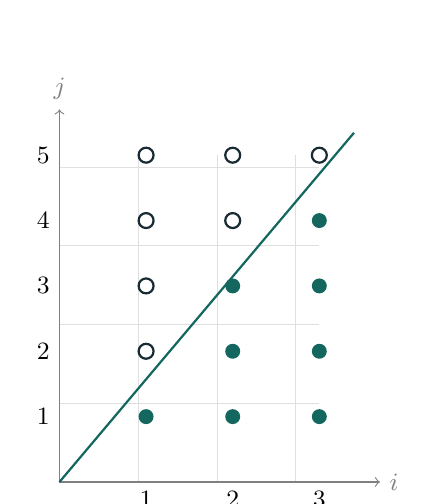
\begin{tikzpicture}[x=1.10cm,y=0.83cm, font=\small]
\draw[very thin,gray!25] (0,0) grid (3,5);
\draw[->,gray] (0,0)--(3.70,0) node[right] {$i$};
\draw[->,gray] (0,0)--(0,5.70) node[above] {$j$};
\draw[accent,thick] (0,0)--(3.40,5.3429);
\foreach \x in {1,2,3}{\node[below] at (\x,0) {\x};}
\foreach \y in {1,2,3,4,5}{\node[left] at (0,\y) {\y};}
\foreach \x in {1,2,3}{\foreach \y in {1,2,3,4,5}{\ifnum\numexpr7*\y\relax<\numexpr11*\x\relax
\fill[accent] (\x,\y) circle (2.7pt);\else
\draw[ink,fill=white,thick] (\x,\y) circle (2.7pt);\fi}}
\end{tikzpicture}
\end{minipage}\hfill
\begin{minipage}[c]{.54\linewidth}
\lab{An instance of the sign change} For $p=7$, $q=11$, there are $3\cdot5=15$ points. The filled points satisfy $7j<11i$. The three columns contribute $1,3,4$, totaling $8$. The five rows contain $0,1,1,2,3$ open points, totaling $7$.

Thus $\leg{11}{7}=+1$ and $\leg{7}{11}=-1$. Indeed $2^2\equiv11\pmod7$, and the squares of $1,2,3,4,5$ modulo $11$ are $1,4,9,5,3$. Both primes are $3\bmod4$.
\end{minipage}

\vspace{7pt}
The diagram depicts integer comparisons. The proof of \eqref{eq:rectangle} uses only the two bounded sums of their indicator functions, the division equation, and the strict bounds above.
\clearpage
\sect{Supplementary laws and witnesses}\label{sec:supp}
For $a=p-1$, the remainders $r_i=p-i$ all exceed $h$. Thus $N_p(p-1)=h$, and Gauss's lemma gives
\begin{equation}\label{eq:minusone}
                 \leg{-1}{p}=(-1)^{(p-1)/2}.
\end{equation}
For $a=2$, $2\le 2i\le p-1$ when $1\le i\le h$, so $r_i=2i$. A remainder is large just when $i>\floor{h/2}$. Consequently $N_p(2)=h-\floor{h/2}$. To compare parities, note that $(p^2-1)/8=h(h+1)/2$. If $h=2t$, subtracting $N_p(2)=t$ from this exponent gives $2t^2$. If $h=2t+1$, subtracting $N_p(2)=t+1$ gives $2t(t+1)$. Both differences are even. We have proved
\begin{equation}\label{eq:two}
                    \leg{2}{p}=(-1)^{(p^2-1)/8}.
\end{equation}
The resulting signs can be read directly from $p$.
\begin{center}
\begin{tabular}{@{}lcccc@{}}\toprule
$p\bmod 8$ & $1$ & $3$ & $5$ & $7$\\\midrule
$\leg{-1}{p}$ & $+1$ & $-1$ & $+1$ & $-1$\\[3pt]
$\leg{2}{p}$ & $+1$ & $-1$ & $-1$ & $+1$\\\bottomrule
\end{tabular}
\end{center}

\lab{Obtaining the promised root} Suppose input information and reciprocity give $\sgnbit_p(q)=0$. The term $x=\rootf(p,q)$ satisfies $x<p$ and $x^2\equiv q\pmod p$ by the prefix invariant of Section~\ref{sec:bounded}. In the opposite branch the same scan proves $\forall x<p\;(x^2\not\equiv q\pmod p)$. Any proposed integer root would reduce to a root in this interval. In particular the ``exactly one'' case of reciprocity gives a decidable exclusive disjunction, with a numerical witness on whichever side succeeds.

There is a shorter witness when $p=4t+3$ and $a$ is a square unit. Compute $x=\remn_p(a^{t+1})$. Now $h=2t+1$, and Euler's criterion gives
\[
                     x^2\equiv a^{2t+2}=a\cdot a^h\equiv a\pmod p.
\]
For $a\equiv0$ take $x=0$. Modular powering, by recursion in the exponent with reduction after each multiplication, is a PR computation.

\lab{The smallest odd prime} When $p=3$ we have $h=1$. In the square case in \eqref{eq:pair} the number of nonfixed pairs is zero, so its empty product is $1$. The second supplement gives $\leg{2}{3}=-1$. These conventions also cover a column with no points below the diagonal.
\clearpage
\sect{Why quantifier-free induction suffices}\label{sec:audit}
A finite statement can still conceal an induction too strong for $\ipra$. Here are the induction formulas used by the human proof. All bounds and parameters are numerical. Write $\mathbf1_{P}$ for the characteristic bit of a displayed bounded test.

\lab{Searching and inverting} For the root scan the three invariants are $w(t)\le t$, $w(t)<t\Rightarrow w(t)^2\equiv a$, and $i<t\land i^2\equiv a\Rightarrow w(t)\le i$. For the inverse in Section~\ref{sec:euler}, one implementation first scans $1\le d<p$ for the first $d$ whose test $\exists t<p\ (ut\equiv d)$ succeeds. Then it scans $t<p$ for the first match for that $d$. Section~\ref{sec:bounded} applies twice. Once selected, $d$ and $t$ are terms, so the remainder argument proving $d=1$ is ordinary first-order reasoning with those parameters.

\lab{Grouping or selecting terms} If $C(i,j)$ denotes an incidence bit and $v(j)$ the weight, use $1$ or $v(j)$ in a product according as $C=0$ or $C=1$. For a row with precisely two entries $r<s$, its prefix product through $t$ is
\[
  \big(\text{if }r\le t\text{ then }v(r)\text{ else }1\big)
  \big(\text{if }s\le t\text{ then }v(s)\text{ else }1\big).
\]
Both sides are PR terms. Induction on $t$ checks the cases $t+1=r$, $t+1=s$, and neither. This also gives the one-entry and empty-row identities by omitting factors. For the pair product in \eqref{eq:pair}, after rows through $t$ the accumulated contribution is $a^{c(t)}P(t)$ modulo $p$, where $c(t)$ counts pair leaders through $t$ and $P(t)$ multiplies fixed entries through $t$. Each row extends this equation by its computed contribution.

\lab{Signs and floors} The prefix form of \eqref{eq:signed} after multiplication is
\[
  a^t\prod_{i=1}^t i\equiv
  (-1)^{\sum_{i=1}^{t} e_i}\prod_{i=1}^t b_i\pmod p
       \qquad(0\le t\le h).
\]
The modular sign is the PR term selecting $1$ or $p-1$ by parity. The parity conversion sums the individual congruences through $t$. The number of entries in a column through $s$ is $\min(s,\floor{qi/p})$ for $0\le s\le k$. Induction uses only a comparison of $s+1$ with the quotient. Additivity and interchange of the resulting two prefix sums were proved in Section~\ref{sec:bounded}.

These equations and their bounded side conditions give quantifier-free induction formulas after Boolean compilation. For example, a bound on all row entries is a scan for a violation with its result compared to the sentinel. Proof parameters such as $p,q,i$ stay free during induction. Universal closure is taken after the numerical implication is proved. Thus \eqref{eq:target} is a theorem of the stated first-order theory.
\clearpage
\sect{The checked Lean development}\label{sec:lean}
The files in \code{lean/} give a complete Lean~4 proof over \code{Nat} of the numerical theorem. They import Lean's standard library. The signed result is \code{QR.legendre\_reciprocity}, and its two supplementary laws are \code{QR.legendre\_neg\_one} and \code{QR.legendre\_two}. In \code{legendre p a}, the first argument is the denominator $p$. The three-valued symbol has type \code{Int}. The natural-valued bit is used only to encode the sign at units.
\begin{center}\small\renewcommand{\arraystretch}{1.12}
\begin{tabular}{@{}>{\raggedright\arraybackslash}p{.33\linewidth}>{\raggedright\arraybackslash}p{.61\linewidth}@{}}\toprule
\textbf{Lean declaration in \code{QR}} & \textbf{Mathematical content}\\\midrule
\code{squareB\_spec} & The terminating Boolean scan reflects $\exists x<p\ (x^2\equiv a)$.\\
\code{leastRoot\_spec} & The extracted root is least and a failed search returns $p$.\\
\code{pair\_product}, \code{two\_fixed\_product} & A duplicate-free finite list decomposes into pairs, with the stated fixed entries removed.\\
\code{wilson\_product}, \code{euler\_criterion} & The full unit product and the power $a^{H(p)}$ modulo $p$.\\
\code{gauss\_power}, \code{gauss} & The signed half-factorial identity and its Legendre-bit consequence.\\
\code{eisenstein}, \code{floor\_sum\_swap} & High counts and floor sums agree modulo $2$. The two floor sums add exactly to $H(p)H(q)$.\\
\code{reciprocity}, \code{fast\_root} & The numerical reciprocity theorem and the root formula for $p\equiv3\pmod4$.\\\bottomrule
\end{tabular}\end{center}

\lab{A small difference between the two proofs} The Lean pair-product lemma removes each encountered pair from a finite list, with the list length bounding the recursion. For a nonsquare it applies this to $x\mapsto a/x$ as on page~\pageref{sec:euler}. For a square $a=r^2$, the code uses an alternative short argument. Multiplication by $r$ permutes the full unit interval. Multiplying the permuted entries yields $r^{p-1}F\equiv F$. Since $F$ is a unit, $r^{p-1}\equiv1$. Thus $a^h\equiv r^{2h}\equiv1$. This is the square branch of \code{euler\_criterion}. The paper's incidence-array argument gives a direct route using only numerical induction in the object theory.

\lab{Reproducing the checks} Run \code{sh lean/check.sh} with Lean~4.19.0 on the path. It builds every standalone module from source in a fresh temporary directory and prints the axiom dependencies of the main endpoints. Run \code{python3 check.py} to exercise the same identities on small inputs. With the default bound $127$, it covers all $1{,}688$ units for $30$ odd primes and all $435$ distinct unordered prime pairs. Lean reports only \code{propext} and \code{Quot.sound} for the main theorems, including the signed reciprocity law and both supplements.

\lab{Formalization status} The standalone development proves statements about Lean natural numbers. The claimed restriction to $\ipra$ is justified by the numerical derivation in Sections~\ref{sec:bounded}--\ref{sec:audit}. The next page gives the actual internal target and the work required to obtain a kernel-checked derivation from the repository's \code{PRAAx}.
\clearpage
\sect{Encoding the derivation in ProveIt}\label{sec:object}
The companion \code{repo/Goal.lean} targets the ProveIt revision given below. It defines a closed formula \code{sentence} of type \code{Fm PTm 0}, with a concrete bounded formula for nonsquareness, a PR term for $S_p(a)$, and the assumptions of the theorem. The object-language goal is
\[
  [\,]\ \vdash_{\mathsf{PRAAx}}\ \texttt{QuadraticReciprocityObject.sentence}.
\]
The repository's \code{half p} computes $\floor{p/2}$, equal to $H(p)$ on odd inputs. Its \code{prime} expresses the divisor condition as a formula. For $2\le d<p$, $d\mid p$ is equivalent to $\remn_d(p)=0$ by division with remainder, so this assumption agrees with the prime scan in \eqref{eq:target}. The bit for $\neg\exists x<p\ (x^2\equiv a)$ agrees with our sentinel test by bounded reflection.

\lab{Derivation plan} Work in the context $\Gamma$ containing the prime, oddness and distinctness assumptions. The supplied assembly takes two instances of \eqref{eq:eisenstein} and one derivation of \eqref{eq:rectangle}.

\textbf{1. Scans and congruences.} Use \code{Core.Division}'s \code{div\_mod} and \code{div\_mod\_unique}. Use \code{Core.Search}'s \code{search\_spec} and \code{search\_found} for a first zero with the bound as sentinel. For a match test $B$, scan $1-[B]$. Pack parameters into one input where a fold requires it. Represent congruence by equality of the two \code{rem} terms. Compile bounded assertions with \code{Foundations.BoundedSyntax}. Apply its companion \code{BoundedSyntaxInduction.induction} to their prefix forms. The repository's \code{euclid\_lemma\_at} also derives prime divisibility of a factor from divisibility of a product.

\textbf{2. The sign formula.} Define $T$, $D$, $b_i$, $e_i$, $N_p(a)$ and the two incidence arrays by the expressions on pages~\pageref{sec:euler}--\pageref{sec:gauss}. Implement their sums/products with \code{Core.MultiSums}. Apply the prefix identities on page~\pageref{sec:audit} to derive Wilson, Euler, and Gauss. For \code{Permutation.prod\_perm} use the zero-based permutation $i\mapsto D(a(i+1))-1$ on $i<h$ and the inverse with $a^{-1}$. Give each map value $0$ outside the interval, so the global range premise holds since $h>0$. The additive permutation identity follows from \code{fubini} on the single-entry array. Summing division equations modulo two gives the two sign-formula instances.

\textbf{3. The rectangle and closure.} Use the two comparison bits in Section~\ref{sec:rectangle}, the cutoff count on page~\pageref{sec:audit}, and \code{Core.Fubini}'s \code{fubini} to derive the rectangle equality in $\Gamma$. The overlay's \code{assemble} uses \code{par\_add}, and \code{close\_from\_counts} introduces the implication and both universal quantifiers. These three input derivations remain to be encoded. The overlay was prepared against the pinned source. Its Lean~4.32.0 project build was unavailable in the verification environment.

\medskip\small
\textbf{Sources.} The statement and supplementary laws are given in \href{https://en.wikipedia.org/wiki/Quadratic_reciprocity}{\emph{Quadratic reciprocity}}. For the Gauss--Eisenstein floor-sum argument see \href{https://crypto.stanford.edu/pbc/notes/numbertheory/quadrecip.html}{Ben Lynn's number theory notes}. The formal systems and module names above refer to \href{https://github.com/VladimirReshetnikov/ProveIt/tree/1e53ba5b26b144afb01bf6774d75cf35f6c760b2/Logic/PrimitiveRecursiveArithmetic}{Vladimir Reshetnikov's ProveIt, PrimitiveRecursiveArithmetic}, revision \code{1e53ba5b26b1}.
\end{document}
